\documentclass[a4paper]{article}
\usepackage{labreport}

\begin{document}

\section{Objective}
The objective is to measure the time constant of an RC circuit in order to verify the calculated values \cite{UNCC-ECE-Dept:2023}.
\section{Equipment Used}

\begin{itemize}
    \item Digital Multimeter
    \item DC Power Supply
    \item Resistor: $20k\Omega$
    \item Capacitor: $2,200 \mu$F
    \item Alligator (Clips) Jumper
\end{itemize}

\section{Experiment Setup}

\begin{enumerate}
    \item Construct the circuit in Figure 10-1\cite{UNCC-ECE-Dept:2023}.
    \begin{figure}[H]\label{fig10-1}
        \begin{center}
            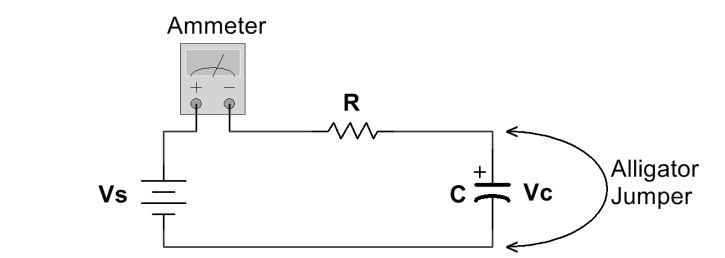
\includegraphics[width = 7 cm]{fig10-1}\\
            \small\textbf{Figure 10-1 Series RC Circuit for Experimental Setup \cite{UNCC-ECE-Dept:2023}}
        \end{center}
    \end{figure} 
    \item Measure the initial current \cite{UNCC-ECE-Dept:2023}.
    \item Calculate the values of $\tau$ and 5$\tau$ in which $\tau$ is equal to $R_{eq}$ times $C_{eq}$ \cite{UNCC-ECE-Dept:2023}.
    \item Collect data by timing the measurements of the current to ever 15 seconds and in order to measure the current remove the alligator clip from the circuit \cite{UNCC-ECE-Dept:2023}.
    \item Take measurements every 15 seconds until 5$\tau$ and possibly further \cite{UNCC-ECE-Dept:2023}.
    \item Repeat the previous 2 steps for trial 2 \cite{UNCC-ECE-Dept:2023}.
    \item Take the average values of the two trials at each measured time \cite{UNCC-ECE-Dept:2023}.
    \item Use the average current to calculate the voltage across the resistor \cite{UNCC-ECE-Dept:2023}.
    \item Solve the voltage across the capacitor, $V_{c}$, which can be solved fro with the voltage accross the resistor $V_{c}$ = ($V_{s}$ - $V_{R}$) \cite{UNCC-ECE-Dept:2023}.  
\end{enumerate}


\section{Results}
$\tau$ = 44 seconds  Initial Current = 1.745 mA  \\
5$\tau$ =  220 seconds \\

\begin{center}
    \small\textbf{Table 10-1: Data Table for RC Time Constant \cite{UNCC-ECE-Dept:2023}}\\
    \begin{tabular}{|p{2 cm}|p{2 cm}|p{2 cm}|p {2 cm}|p {2 cm}|p{2 cm}|}
        \hline
        Time (min:sec) & \multicolumn{3}{|c|}{Current (mA)} & Resistor Voltage (V) & Capacitor Voltage (V) \\
        \hline
        & Trial 1 & Trial 2 & Average & & \\
        \hline
        0:00 & 1.745 mA & 1.745 mA & 1.745 mA & 34.9 V  & 0 V \\
        \hline
        0:15 & 1.242 mA & 1.24 mA & 1.241 mA & 24.82 V & 10.08 V \\
        \hline
        0:30 & .901 mA & .900 mA & .9005 mA & 18.01 V &  16.86 V \\
        \hline
        0:45 & .662 mA & .666 mA & .664 mA & 13.28 V & 21.62 V \\
        \hline
        1:00 & .490 mA & .500 mA & .495 mA & 9.9 V & 25 V \\
        \hline
        1:15 & .365 mA & .373 mA & .369 mA & 7.38 V & 27.52 V \\
        \hline
        1:30 & .277 mA & .274 mA & .2755 mA & 5.51 V & 29.39 V \\
        \hline
        1:45 & .212 mA & .207 mA & .2095 mA & 4.19 V & 30.71 V \\
        \hline
        2:00 & .165 mA & .158 mA & .1615 mA & 3.23 V & 31.67 V \\
        \hline
        2:15 & .125 mA & .112 mA & .1185 mA & 2.37 V & 32.53 V \\
        \hline
        2:30 & .100 mA & .092 mA & .096 mA & 1.92 V & 32.98 V \\
        \hline
        2:45 & .076 mA & .072 mA & .074 mA & 1.48 V & 33.42 V \\
        \hline
        3:00 & .062 mA & .057 mA & .0595 mA & 1.19 V & 33.71 V \\
        \hline
        3:15 & .050 mA & .045 mA & .0475 mA & .95 V & 33.95 V \\
        \hline
        3:30 & .041 mA & .036 mA & .0385 mA & .77 V & 34.13 V \\
        \hline
        3:45 & .034 mA & .029 mA & .0315 mA & .63 V & 34.27 V \\
        \hline
        4:00 & .028 mA & .024 mA & .026 mA & .52 V & 34.38 V \\
        \hline
        4:15 & .023 mA & .020 mA & .0215 mA & .43 V & 34.47 V \\
        \hline
        4:30 & .020 mA & .016 mA & .018 mA & .36 V & 34.54 V \\
        \hline
        4:45 & .017 mA & .014 mA & .0155 mA & .31 V & 34.59 V \\
        \hline
        5:00 & .015 mA & .012 mA & .0135 mA & .27 V & 34.63 V \\
        \hline
        5:15 & .013 mA & .010 mA & .0115 mA & .23 V & 34.67 V \\
        \hline
        5:30 & .011 mA & .009 mA & .010 mA & .2 V & 34.7 V \\
        \hline
        5:45 & .010 mA & .008 mA & .009 mA & .18 V & 34.72 V \\
        \hline
        6:00 & .009 mA & .007 mA & .008 mA & .16 V & 34.74 V \\
        \hline
    \end{tabular}
\end{center}



\section{Conclusion}



\bibliography{references}
\bibliographystyle{plain}



\end{document}